\begin{center}
    % Gain
    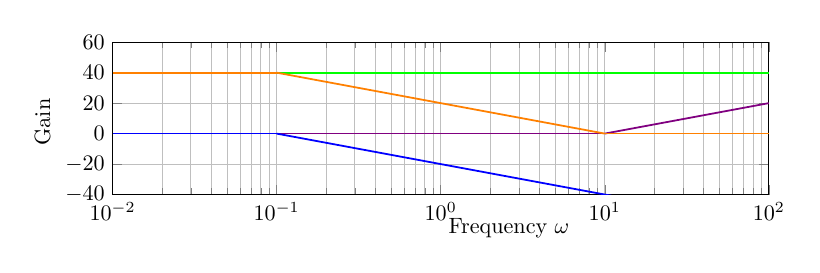
\begin{tikzpicture}
        [
            scale = 0.8,
            >=latex
        ]
        \begin{axis}
            [
                width=12cm,
                height=4cm,
                xmode=log,
                xmin=0.01, xmax=100, ymin=-40, ymax=60,
                x label style={anchor=west},
                xlabel=Frequency $\omega$,
                y label style={anchor=south},
                ylabel=Gain $\deci \bel$,
                xmajorgrids=true,
                xminorgrids=true,
                ymajorgrids=true
            ]

            % K_0
            \addplot[thick, color=green, domain=0.01:100]{40};

            % Nullstelle
            \addplot[thick, color=violet, domain=0.01:10]{0};               % start bis Knick
            \addplot[thick, color=violet, domain=10:100]{20*log10(x)-20};   % ab Knick nach oben    

            % Polstelle
            \addplot[thick, color=blue, domain=0.01:0.1]{0};                % start bis Knick
            \addplot[thick, color=blue, domain=0.1:100]{-20*log10(x)-20};   % ab Knick nach oben    
            
            % Grafische Addition
            \addplot[thick, color=orange, domain=0.01:0.1]{40};    
            \addplot[thick, color=orange, domain=0.1:10]{-20*log10(x)+20};        
            \addplot[thick, color=orange, domain=10:100]{0};      
           
        \end{axis}
        
    \end{tikzpicture}


    % Phase
    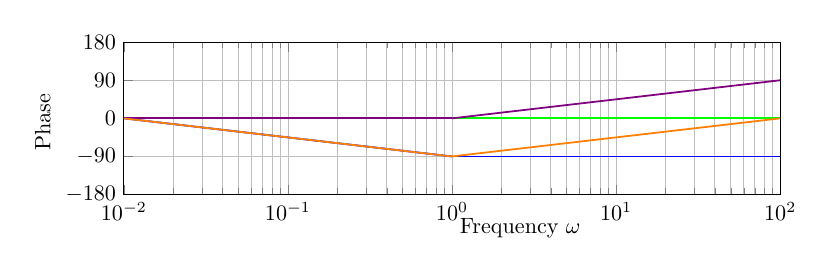
\begin{tikzpicture}
        [
            scale = 0.8,
            >=latex
        ]
        \begin{axis}
            [
                width=12cm,
                height=4cm,
                xmode=log,
                xmin=0.01, xmax=100, ymin=-180, ymax=180,
                x label style={anchor=west},
                xlabel=Frequency $\omega$,
                y label style={anchor=south},
                ylabel=Phase $\degree$,
                ytick={-180, -90, 0, 90, 180},
                % yticklabels={-180, -90, 0, 90, 180},
                xmajorgrids=true,
                xminorgrids=true,
                ymajorgrids=true
            ]
            
            % K_0
            \addplot[thick, color=green, domain=0.01:100]{0};
                
            % Nullstelle
            \addplot[thick, color=violet, domain=0.01:1]{0};              % start bis Knick
            \addplot[thick, color=violet, domain=1:100]{45*log10(x)};     % ab Knick nach oben    
            
            % Polstelle
            \addplot[thick, color=blue, domain=0.01:1]{-45*log10(x)-90};    % start bis Knick
            \addplot[thick, color=blue, domain=1:100]{-90};                 % ab Knick gerade
            
            % Grafische Addition
            \addplot[thick, color=orange, domain=0.01:1]{-45*log10(x)-90};    
            \addplot[thick, color=orange, domain=1:100]{45*log10(x)-90};           


            
        \end{axis}
            
    \end{tikzpicture}
\end{center}